\subsection{Mašīnmācīšanās modelis}

    Mašīnmācīšanās modeļa izstrādi ir iespējams sadalīt vēl divās daļās: modeļa trenēšana un modeļa
    implementācija tīmekļa aplikācijā.

    Sākotnēji tika veikta izpēte par to, kādi gatavi
    ietvari jau eksistē \texttt{C\#} ekosistēmā. Tika atrasti tādi ietvari, kā \texttt{PyTorch.NET},
    \texttt{Keras.NET}, \texttt{ML.NET} un \texttt{CNTK}. Sākumā bija plānots izmantot \texttt{CNTK},
    bet izpētes processā tika secināts, ka Microsoft ir pārtraukuši atbalstu \texttt{CNTK} un vairs
    to neuzlabos un neatjaunos \cite{chrisbasogluCNTKReleaseNotes}. Šī iemesla dēļ tika izvēlēts \texttt{ML.NET} ietvars.

    Attiecīgi tika izveidota programma, kas apmāca modeli, izmantojot \texttt{MNIST} datu kopu, un
    šīs programmas darbība ir aprakstīta \ref{ml:train}~attēlā. Kā piemēri tika izmantoti citi jau
    eksistējoši \texttt{GithHub} projekti un \texttt{ML.NET} un \texttt{MNIST} dokumentācija.
    \cite{DotnetMachinelearningsamples2021} \cite{kexugitTestRunWorking} \cite{MLNETTutorial}
    \cite{natkeMLNETDocumentation} \cite{paxbunPaxbunCntkMnistPractice2019}

    \begin{figure}[H]
        \centering
        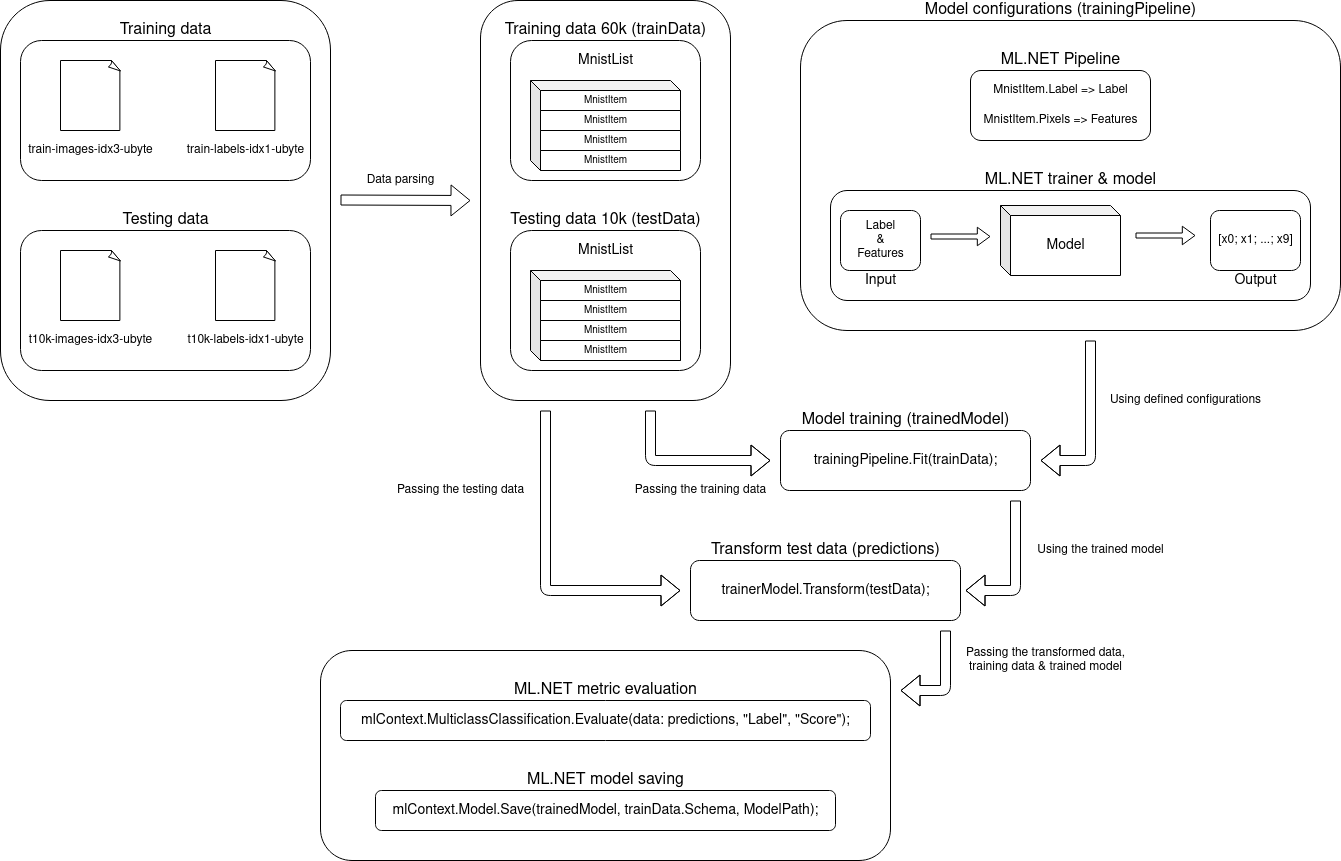
\includegraphics[width=15cm]{VPL-ML.png}
        \caption{ML modeļa trenēšanas diagramma}
        \label{ml:train}
    \end{figure}

    Sākumā tika iegūti \texttt{MNIST} dati no "THE MNIST DATABASE" \cite{MNISTHandwrittenDigit}. Tie ir
    4 bināri faili un tos diagrammā var redzēt "Training data" un "Testing data" kvadrātos. Pēc datu iegūšanas
    tika izveidots datu parsēšanas funkcija, kas ielasa visus datus atmiņā un sadala tos pa klasēm \texttt{MnistList} un \texttt{MnistItem}. Izmantojot \texttt{ML.NET}, tiek nodefinēta
    konfigurācija prieks \texttt{ML.NET} "pipeline". Konfigurācijā ietilpst mainīgo sasaistīšana un
    modeļa veida definēšana. Pēc konfigurācijas definēšanas un datu ielasīšanas tiek trenēts modelis
    izmantojot \texttt{.Fit()} metodi. Ir nepieciešams pārbaudīt cik labi šis
    modelis ir uztrenēts, tāpēc tiek veiktas transformācijas uz datiem, kuri iepriekš ir izmantoti modeļā trenēšanai. Tas tiek veikts, izmantojot \texttt{.Transform()} metodi. Pēc šis pārbaudes ar \texttt{.Evaluate()} metodi modelis tiek izvērtēts. Pēdējais solis ir to saglabāt. Tas tiek izdarīts
    izmantojot \texttt{.Save()} metodi.

    Rezultātā tika iegūts modelis, kuru metriku rezultāti ir redzami \ref{ml:metrics}~attēlā.

    \begin{figure}[H]
        \centering
        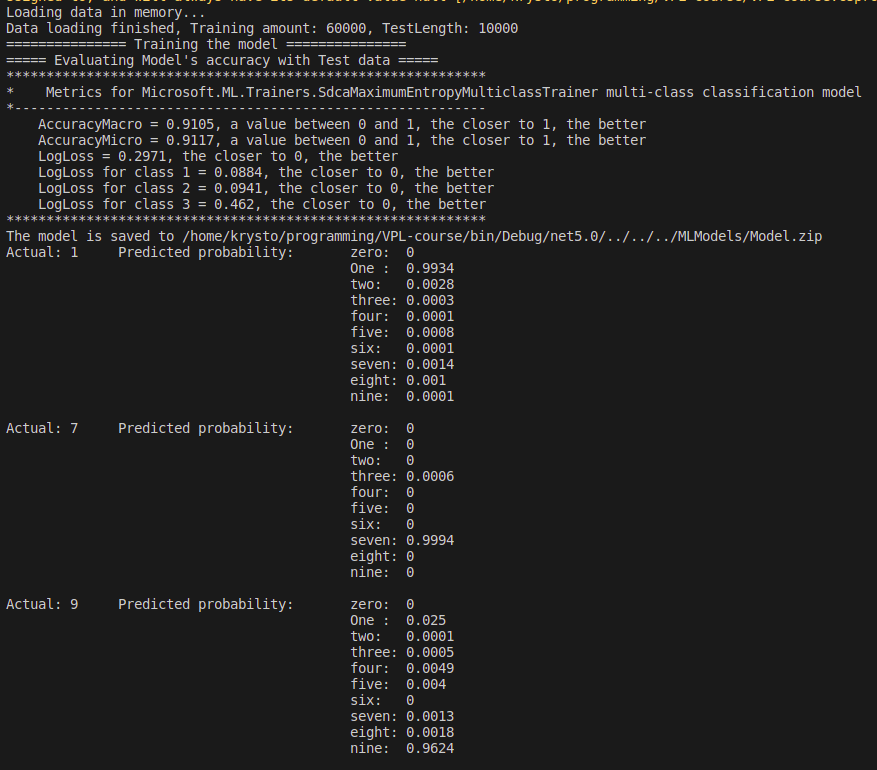
\includegraphics[width=13cm]{training-sc-v2.png}
        \caption{ML modeļa metriku rezultāti}
        \label{ml:metrics}
    \end{figure}

    Kad modelis bija izveidots, tad to bija nepieciešams implementēt tīmekļa aplikācijā. Tika izveidota
    \texttt{MnistClassificator} klase, kurā atrodas  metode \mintinline{csharp}{public float[] Analyze(byte[] image)}, kas tiek padota izveidotam modelim, kas atgriež
    virkni ar float vērtībām. Šīs vērtības reprezentē procentuālās vērtības ciparu klasēm.
